\immediate\write18{tex spath.dtx}
\documentclass{standalone}
\usepackage{tikz}
\usetikzlibrary{decorations}
\usepackage{spath}

\begin{document}
\begin{tikzpicture}
\useasboundingbox (-5,-5) rectangle (5,5);
\path[decoration={curveto},decorate,save path=\tmppath] (2,0) to[bend right] (4,2) to[bend right] (5,0) to[bend right] (2,0);
\pgfoonew \opath=new spath(\tmppath)
\opath.prepare()
\opath.spirograph(,0pt,0pt,36)
\opath.use path with tikz(draw,blue)
\end{tikzpicture}
\end{document}



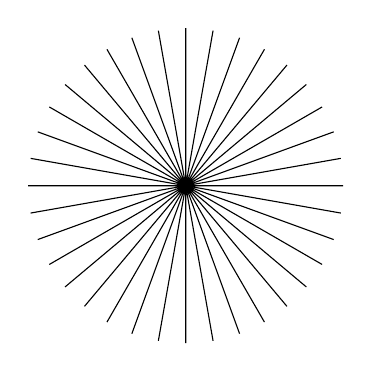
\begin{tikzpicture}
\draw[save path=\tmppath] \foreach \k in {0,...,1000} {(0,0) -- +(\k * 10:2)};
\pgfoonew \mypath=new spath(\tmppath)
\mypath.prepare()
\mypath.initial point()
\mypath.final point()
\end{tikzpicture}
\end{document}
\draw[save path=\tmppath,line width=1mm,red] (-1,0) -- (0,0) .. controls +(1,0) and +(1,0) .. (1,1);
%\path[save path=\tmppath] (-1,0) .. controls +(.1,0) and +(-.1,0) .. (0,1) .. controls +(.1,0) and +(-.1,0) .. (1,0);
\show\tmppath
\pgfoonew \mypath=new spath(\tmppath)
\mypath.prepare()
\mypath.show(path)
\mypath.reverse path()
\mypath.show(path)
\mypath.use path with tikz(draw)
\mypath.translate path(,0cm,-2cm)
\mypath.at least three()
\mypath.show(path)
\mypath.show(real length)
\mypath.split path by real length(\fpath,\mpath,1)
\begin{scope}[ultra thick]
\fpath.taper out()
\fpath.use path with tikz(fill)
\mpath.split path by real length(\mmpath,\epath,-1)
\epath.reverse path()
\epath.taper out()
\epath.use path with tikz(fill)
\mmpath.use path with tikz(draw)
\end{scope}
%\mypath.show(reverse path)

%\fpath.show(reverse path)
%\epath.show(reverse path)
\end{tikzpicture}
\end{document}


\begin{tikzpicture}
\path[save path=\tmppath] (0,0) -- (1,1) (2,1) .. controls (3,1) and (4,2) .. (5,2);
\show\tmppath
\pgfoonew \mypath =new spath(\tmppath)
\mypath.show(path)
\mypath.length()
\mypath.initial point()
\mypath.show(initial point)
\mypath.final point()
\mypath.show(final point)
\mypath.show(length)
\mypath.translate path(\trpath,1cm,1cm)
\mypath.show(path)
\trpath.show(path)
\mypath.concatenate(\catpath,\trpath)
\catpath.show(path)
\mypath.weld(,\trpath)
\mypath.show(path)
\mypath.use path with tikz(draw,red,line width=.5cm)
\mypath.use path(stroke)
\pgfsetlinewidth{5pt}
\mypath.show(length)
\mypath.set(taper line width,2pt)
\mypath.translate path(,0pt,-1cm)
\mypath.prepare()
\mypath.show(first action)
\mypath.taper start(\taperpath,\restpath)
\taperpath.show(path)
\taperpath.use path(fill)
\restpath.taper end(\taperendpath,\morepath)
\taperendpath.use path(fill)
\morepath.use path(stroke)
\mypath.show(path)
\end{tikzpicture}
\end{document}
\show\tmppath
\spathsplit\mysplitpath\tmppath
\mysplitpath.get path(\firstpath)
\firstpath.show attribute(path)
\mysplitpath.get next component(\mynextbit)
\mynextbit.get path(\otherpath)
\otherpath.translate(,-1cm,0pt)
\firstpath.concatenate(\otherpath,\catpath)
\otherpath.show attribute(path)
\firstpath.show attribute(path)
\catpath.show attribute(path)
\pgfsetstrokecolor{red}
%\otherpath.use path(stroke)
\mynextbit.get path(\otherpath)
\otherpath.show attribute(reverse)
\otherpath.prepare()
\otherpath.show attribute(reverse)
\otherpath.show attribute(path)
\pgfsetstrokecolor{blue}
\otherpath.use path(stroke)
%\otherpath.use path(stroke)
\otherpath.at least three()
\otherpath.show attribute(path)
\otherpath.translate(,0pt,1cm)
\pgfsetstrokecolor{red}
\pgfsetfillcolor{red}
\pgfsetlinewidth{.1cm}
\otherpath.taper start(\taperpath,\restpath)
\taperpath.show attribute(path)
\taperpath.use path(fill)
\restpath.taper end(\taperendpath,\morepath)
\taperendpath.use path(fill)
\morepath.use path(stroke)
\end{tikzpicture}
\end{document}

\begin{document}
\begin{tikzpicture}
\draw[save path=\tmppath] (0,0) -- (1,1) (2,1) .. controls (3,1) and (4,2) .. (5,2);
\makeatletter
\show\tmppath
\spath@translate\tmppath{1cm}{0cm}
\show\spath@tmppath
\spath@start\spath@tmppath
\showthe\spath@sx
\showthe\spath@sy
\spath@length\tmppath
\message{Length: \arabic{spath@length}}
\spath@components\tmppath
\message{Components: \arabic{spath@length}}
\spath@reverse\tmppath
\show\spath@tmppath
\spath@start\tmppath
\showthe\spath@sx
\showthe\spath@sy
\spath@end\tmppath
\showthe\spath@ex
\showthe\spath@ey
\show\tmppath
\spath@prepare\tmppath{path}
\show\spath@array@path@length
\expandafter\show\csname spath@array@path@1\endcsname
\expandafter\show\csname spath@array@path@1@rev\endcsname
\expandafter\show\csname spath@array@path@1@start\endcsname
\expandafter\show\csname spath@array@path@1@end\endcsname
\expandafter\show\csname spath@array@path@1@length\endcsname
\expandafter\show\csname spath@array@path@1@first\endcsname
\expandafter\show\csname spath@array@path@1@last\endcsname
\expandafter\show\csname spath@array@path@2\endcsname
\expandafter\show\csname spath@array@path@2@rev\endcsname
\expandafter\show\csname spath@array@path@2@start\endcsname
\expandafter\show\csname spath@array@path@2@end\endcsname
\expandafter\show\csname spath@array@path@2@length\endcsname
\expandafter\show\csname spath@array@path@2@first\endcsname
\expandafter\show\csname spath@array@path@2@last\endcsname
\makeatother
\end{tikzpicture}
\end{document}

% Local Variables:
% tex-output-type: "pdf18"
% End: